\setcounter{definition}{0} \setcounter{property}{0} \setcounter{claim}{0} \setcounter{fact}{0} \setcounter{corollary}{0} \setcounter{figure}{0}

\section{Closest Pair Problem}

Given a set of $n$ points in 2D plane, $P = \{p_1, p_2, \cdots, p_n\}$, where each point $p_i$ is
represented as its $x$-coordinate $p_i.x$ and $y$-coordinate $p_i.y$, the \emph{closest pair}
problem seeks a pair of points $p_i, p_j \in P$ such that their distance, 
defined as $dist(p_i, p_j) = \sqrt{(p_i.x - p_j.x)^2 + (p_i.y - p_j.y)^2}$,
is minimized.

\begin{figure}[h!]
\centering{

\tikzset{every picture/.style={line width=0.75pt}} %set default line width to 0.75pt        

\begin{tikzpicture}[x=0.5pt,y=0.5pt,yscale=-1,xscale=1]
%uncomment if require: \path (0,312); %set diagram left start at 0, and has height of 312

%Flowchart: Connector [id:dp3585002987789013] 
\draw  [fill={rgb, 255:red, 0; green, 0; blue, 0 }  ,fill opacity=1 ] (246.06,175.88) .. controls (243.68,176.34) and (241.39,174.78) .. (240.94,172.41) .. controls (240.49,170.03) and (242.04,167.74) .. (244.42,167.29) .. controls (246.79,166.83) and (249.08,168.39) .. (249.54,170.77) .. controls (249.99,173.14) and (248.43,175.43) .. (246.06,175.88) -- cycle ;
%Flowchart: Connector [id:dp7980412079509043] 
\draw  [fill={rgb, 255:red, 0; green, 0; blue, 0 }  ,fill opacity=1 ] (65.58,122.88) .. controls (63.2,123.34) and (60.91,121.78) .. (60.46,119.41) .. controls (60,117.03) and (61.56,114.74) .. (63.94,114.29) .. controls (66.31,113.83) and (68.6,115.39) .. (69.05,117.77) .. controls (69.51,120.14) and (67.95,122.43) .. (65.58,122.88) -- cycle ;
%Flowchart: Connector [id:dp9736868983859984] 
\draw  [fill={rgb, 255:red, 0; green, 0; blue, 0 }  ,fill opacity=1 ] (184.62,17.88) .. controls (182.25,18.34) and (179.95,16.78) .. (179.5,14.41) .. controls (179.05,12.03) and (180.6,9.74) .. (182.98,9.29) .. controls (185.35,8.83) and (187.64,10.39) .. (188.1,12.77) .. controls (188.55,15.14) and (186.99,17.43) .. (184.62,17.88) -- cycle ;
%Flowchart: Connector [id:dp957649299032159] 
\draw  [fill={rgb, 255:red, 0; green, 0; blue, 0 }  ,fill opacity=1 ] (272.64,108.88) .. controls (270.27,109.34) and (267.98,107.78) .. (267.52,105.41) .. controls (267.07,103.03) and (268.63,100.74) .. (271,100.29) .. controls (273.37,99.83) and (275.67,101.39) .. (276.12,103.77) .. controls (276.57,106.14) and (275.02,108.43) .. (272.64,108.88) -- cycle ;
%Flowchart: Connector [id:dp6348640590918235] 
\draw  [fill={rgb, 255:red, 0; green, 0; blue, 0 }  ,fill opacity=1 ] (393.64,152.88) .. controls (391.27,153.34) and (388.98,151.78) .. (388.52,149.41) .. controls (388.07,147.03) and (389.63,144.74) .. (392,144.29) .. controls (394.37,143.83) and (396.67,145.39) .. (397.12,147.77) .. controls (397.57,150.14) and (396.02,152.43) .. (393.64,152.88) -- cycle ;
%Flowchart: Connector [id:dp9650319562783608] 
\draw  [fill={rgb, 255:red, 0; green, 0; blue, 0 }  ,fill opacity=1 ] (373.64,38.88) .. controls (371.27,39.34) and (368.98,37.78) .. (368.52,35.41) .. controls (368.07,33.03) and (369.63,30.74) .. (372,30.29) .. controls (374.37,29.83) and (376.67,31.39) .. (377.12,33.77) .. controls (377.57,36.14) and (376.02,38.43) .. (373.64,38.88) -- cycle ;
%Flowchart: Connector [id:dp1191629503329028] 
\draw  [fill={rgb, 255:red, 0; green, 0; blue, 0 }  ,fill opacity=1 ] (89.64,252.88) .. controls (87.27,253.34) and (84.98,251.78) .. (84.52,249.41) .. controls (84.07,247.03) and (85.63,244.74) .. (88,244.29) .. controls (90.37,243.83) and (92.67,245.39) .. (93.12,247.77) .. controls (93.57,250.14) and (92.02,252.43) .. (89.64,252.88) -- cycle ;
%Flowchart: Connector [id:dp46368149090735455] 
\draw  [fill={rgb, 255:red, 0; green, 0; blue, 0 }  ,fill opacity=1 ] (368.62,253.88) .. controls (366.25,254.34) and (363.95,252.78) .. (363.5,250.41) .. controls (363.05,248.03) and (364.6,245.74) .. (366.98,245.29) .. controls (369.35,244.83) and (371.64,246.39) .. (372.1,248.77) .. controls (372.55,251.14) and (370.99,253.43) .. (368.62,253.88) -- cycle ;
%Flowchart: Connector [id:dp6008165035231083] 
\draw  [fill={rgb, 255:red, 0; green, 0; blue, 0 }  ,fill opacity=1 ] (266.64,282.88) .. controls (264.27,283.34) and (261.98,281.78) .. (261.52,279.41) .. controls (261.07,277.03) and (262.63,274.74) .. (265,274.29) .. controls (267.37,273.83) and (269.67,275.39) .. (270.12,277.77) .. controls (270.57,280.14) and (269.02,282.43) .. (266.64,282.88) -- cycle ;
%Flowchart: Connector [id:dp08654676996934618] 
\draw  [fill={rgb, 255:red, 0; green, 0; blue, 0 }  ,fill opacity=1 ] (167.64,120.84) .. controls (165.27,121.29) and (162.98,119.73) .. (162.52,117.36) .. controls (162.07,114.99) and (163.63,112.69) .. (166,112.24) .. controls (168.37,111.79) and (170.67,113.34) .. (171.12,115.72) .. controls (171.57,118.09) and (170.02,120.38) .. (167.64,120.84) -- cycle ;

% Text Node
\draw (264,110.45) node [anchor=north west][inner sep=0.75pt]   [align=left] {$\displaystyle p_{6}$};
% Text Node
\draw (175,19.45) node [anchor=north west][inner sep=0.75pt]   [align=left] {$\displaystyle p_{2}$};
% Text Node
\draw (237,177.45) node [anchor=north west][inner sep=0.75pt]   [align=left] {$\displaystyle p_{1}$};
% Text Node
\draw (365,40.45) node [anchor=north west][inner sep=0.75pt]   [align=left] {$\displaystyle p_{7}$};
% Text Node
\draw (81,254.45) node [anchor=north west][inner sep=0.75pt]   [align=left] {$\displaystyle p_{3}$};
% Text Node
\draw (384.52,154.45) node [anchor=north west][inner sep=0.75pt]   [align=left] {$\displaystyle p_{5}$};
% Text Node
\draw (56,124.45) node [anchor=north west][inner sep=0.75pt]   [align=left] {$\displaystyle p_{4}$};
% Text Node
\draw (359,255.45) node [anchor=north west][inner sep=0.75pt]   [align=left] {$\displaystyle p_{8}$};
% Text Node
\draw (258,284.45) node [anchor=north west][inner sep=0.75pt]   [align=left] {$\displaystyle p_{9}$};
% Text Node
\draw (159,122.41) node [anchor=north west][inner sep=0.75pt]   [align=left] {$\displaystyle p_{10}$};


\end{tikzpicture}

}
\caption{A set of 2D points $P = \{p_1, p_2, \cdots, p_{9}, p_{10}\}$.
The closest pair is $(p_1, p_6)$.}
\label{fig:2d}
\end{figure}


A brute-force algorithm enumerates all pairs, compute their distances,
and find the smallest one: 

\begin{minipage}{0.8\textwidth}
	\aaA {9}{Algorithm~\#1~($P[1\cdots n]$)}\xxx
	\aab {use $d^*$ to store the current minimum distance, initialized as a large number $M$}\xxx
	\aab {use $(p^*, q^*)$ to store the corresponding optimal pair, initialized as NULL}\xxx
	\aaB {5}{for $i=1$ to $n$}\xxx
	\aaC {3}{for $j=i+1$ to $n$}\xxx
	\aad {$d = dist(P[i], P[j])$;}\xxx
	\aad {if $d < d^*$: $d^* = d$, $p^* = P[i]$, $q^* = P[j]$; }\xxx
	\aac {end}\xxx
	\aab {end}\xxx
	\aaa {end algorithm;}\xxx
\end{minipage}

The above algorithm certainly takes $\Theta(n^2)$ time.
We aim for designing a faster, $\Theta(n\cdot \log n)$ algorithm.
To achieve this, we certainly need to avoid the above all-vs-all comparisons.
How? Let's consider the 1D closest pair problem, i.e., the given $n$ points $P = \{p_1, p_2, \cdots, p_n\}$
all locate on the $x$-axis~(now each point is represented by a single coordinate rather than two coordinates).
See the example below.
To find the closest pair, we can sort all points from left to right. Let $P' = (p'_1, p'_2, \cdots, p'_n)$ be the
sorted list of these 1D points. It is obvious that the closest pair of $P$ must be adjacent in $P'$, i.e.,
the closest pair must be $(p'_i, p'_{i+1})$ for some $i$. Hence, we can compute $dist(p'_i, p'_{i+1})$ for
all $1\le i \le n - 1$ and pick the minimum. The whole process takes $\Theta(n\log n)$ time as the sorting
step takes $\Theta(n\log n)$ time and the following step takes $\Theta(n)$ time.

\begin{figure}[h!]
\centering{\tikzset{every picture/.style={line width=0.75pt}} %set default line width to 0.75pt        

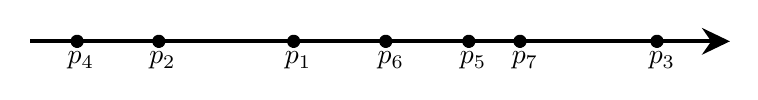
\begin{tikzpicture}[x=0.5pt,y=0.5pt,yscale=-1,xscale=1]
%uncomment if require: \path (0,73); %set diagram left start at 0, and has height of 73

%Flowchart: Connector [id:dp7323125525690383] 
\draw  [fill={rgb, 255:red, 0; green, 0; blue, 0 }  ,fill opacity=1 ] (269.06,32.88) .. controls (266.68,33.34) and (264.39,31.78) .. (263.94,29.41) .. controls (263.49,27.03) and (265.04,24.74) .. (267.42,24.29) .. controls (269.79,23.83) and (272.08,25.39) .. (272.54,27.77) .. controls (272.99,30.14) and (271.43,32.43) .. (269.06,32.88) -- cycle ;
%Flowchart: Connector [id:dp43205645238132784] 
\draw  [fill={rgb, 255:red, 0; green, 0; blue, 0 }  ,fill opacity=1 ] (112.58,32.88) .. controls (110.2,33.34) and (107.91,31.78) .. (107.46,29.41) .. controls (107,27.03) and (108.56,24.74) .. (110.94,24.29) .. controls (113.31,23.83) and (115.6,25.39) .. (116.05,27.77) .. controls (116.51,30.14) and (114.95,32.43) .. (112.58,32.88) -- cycle ;
%Flowchart: Connector [id:dp18857411746512043] 
\draw  [fill={rgb, 255:red, 0; green, 0; blue, 0 }  ,fill opacity=1 ] (171.62,32.88) .. controls (169.25,33.34) and (166.95,31.78) .. (166.5,29.41) .. controls (166.05,27.03) and (167.6,24.74) .. (169.98,24.29) .. controls (172.35,23.83) and (174.64,25.39) .. (175.1,27.77) .. controls (175.55,30.14) and (173.99,32.43) .. (171.62,32.88) -- cycle ;
%Straight Lines [id:da6345715509082558] 
\draw [color={rgb, 255:red, 0; green, 0; blue, 0 }  ,draw opacity=1 ][line width=1.5]    (579.52,28.59) -- (77.52,28.59) ;
\draw [shift={(583.52,28.59)}, rotate = 180] [fill={rgb, 255:red, 0; green, 0; blue, 0 }  ,fill opacity=1 ][line width=0.08]  [draw opacity=0] (20.36,-9.78) -- (0,0) -- (20.36,9.78) -- (13.52,0) -- cycle    ;
%Flowchart: Connector [id:dp4623670345777464] 
\draw  [fill={rgb, 255:red, 0; green, 0; blue, 0 }  ,fill opacity=1 ] (335.64,32.88) .. controls (333.27,33.34) and (330.98,31.78) .. (330.52,29.41) .. controls (330.07,27.03) and (331.63,24.74) .. (334,24.29) .. controls (336.37,23.83) and (338.67,25.39) .. (339.12,27.77) .. controls (339.57,30.14) and (338.02,32.43) .. (335.64,32.88) -- cycle ;
%Flowchart: Connector [id:dp49328940914196706] 
\draw  [fill={rgb, 255:red, 0; green, 0; blue, 0 }  ,fill opacity=1 ] (395.64,32.88) .. controls (393.27,33.34) and (390.98,31.78) .. (390.52,29.41) .. controls (390.07,27.03) and (391.63,24.74) .. (394,24.29) .. controls (396.37,23.83) and (398.67,25.39) .. (399.12,27.77) .. controls (399.57,30.14) and (398.02,32.43) .. (395.64,32.88) -- cycle ;
%Flowchart: Connector [id:dp6321121302385494] 
\draw  [fill={rgb, 255:red, 0; green, 0; blue, 0 }  ,fill opacity=1 ] (432.64,32.88) .. controls (430.27,33.34) and (427.98,31.78) .. (427.52,29.41) .. controls (427.07,27.03) and (428.63,24.74) .. (431,24.29) .. controls (433.37,23.83) and (435.67,25.39) .. (436.12,27.77) .. controls (436.57,30.14) and (435.02,32.43) .. (432.64,32.88) -- cycle ;
%Flowchart: Connector [id:dp3584547063985092] 
\draw  [fill={rgb, 255:red, 0; green, 0; blue, 0 }  ,fill opacity=1 ] (531.64,32.88) .. controls (529.27,33.34) and (526.98,31.78) .. (526.52,29.41) .. controls (526.07,27.03) and (527.63,24.74) .. (530,24.29) .. controls (532.37,23.83) and (534.67,25.39) .. (535.12,27.77) .. controls (535.57,30.14) and (534.02,32.43) .. (531.64,32.88) -- cycle ;

% Text Node
\draw (327,34.45) node [anchor=north west][inner sep=0.75pt]   [align=left] {$\displaystyle p_{6}$};
% Text Node
\draw (162,34.45) node [anchor=north west][inner sep=0.75pt]   [align=left] {$\displaystyle p_{2}$};
% Text Node
\draw (260,34.45) node [anchor=north west][inner sep=0.75pt]   [align=left] {$\displaystyle p_{1}$};
% Text Node
\draw (424,34.45) node [anchor=north west][inner sep=0.75pt]   [align=left] {$\displaystyle p_{7}$};
% Text Node
\draw (523,34.45) node [anchor=north west][inner sep=0.75pt]   [align=left] {$\displaystyle p_{3}$};
% Text Node
\draw (386.52,34.45) node [anchor=north west][inner sep=0.75pt]   [align=left] {$\displaystyle p_{5}$};
% Text Node
\draw (103,34.45) node [anchor=north west][inner sep=0.75pt]   [align=left] {$\displaystyle p_{4}$};


\end{tikzpicture}
}
\caption{A set of 1D points $P = \{p_1, p_2, \cdots, p_{7}\}$.
After sorting we get $P' = (p_4, p_2, p_1, p_6, p_5, p_7, p_3)$, 
and the closest pair must be next to each other in $P'$; in this case it is $(p_5, p_7)$.}
\end{figure}

For 1D closest pair problem, after sorting one point $p_i$ only needs to be compared with one other point~(i.e.,
its successor in the sorted list $P'$). We will try to borrow these ideas to the 2D case. 
That is, we will try to sort the points~(in some way), and we hope to show that it suffices to compare one point
to constant number of other points. Such extension to 2D case is by no means obvious though.

We now design a divide-and-conquer algorithm, aiming for achieving a time complexity of $\Theta(n\log n)$.
In a preprocessing step, we sort all points in $P$ according to their $x$-coordinates in ascending order, obtaining a sorted list denoted as $P_X$.
We will also sort all points according to their $y$-coordinates in ascending order, obtaining a sorted list denoted as $P_Y$.
For example in Figure~\ref{fig:2d}, $P_X = (p_4, p_3, p_{10}, p_2, p_1, p_9, p_6, p_8, p_7, p_5)$, and
$P_Y = (p_9, p_8, p_3, p_1, p_5, p_4, p_{10}, p_6, p_7, p_2)$.
You will see later, that we need both sorted lists.

Since we design a divide-and-conquer algorithm, we need to define the recursive function.
We define DC-closest-pair~($P_X, P_Y$), where $P_X$ and $P_Y$ are the sorted lists of the same set of points $P$
w.r.t.~$x$- and $y$-coordinates, returns the closest pair $(p^*, q^*)$ in $P$.
We follow the framework of divide-and-conquer, that partitions the input into smaller subproblems.
Naturally, we can partition the points in $P$ into two halves, $L$ and $R$,
based on their $x$-coordinates.  
For example in Figure~\ref{fig:2d}, we
will have $L = \{p_1, p_2, p_3, p_4, p_{10}\}$ and $R = \{p_5, p_6, p_7, p_8, p_9\}$.
Note that, in order to recursively call DC-closest-pair on $L$ and $R$, we have
to create the corresponding sorted lists for both $L$ and $R$.  That is, for
the left partition $L$, we have to create $L_X$ and $L_Y$, the sorted lists of
$L$ w.r.t.~$x$- and $y$-coordinates, and for $R$ we need to create $R_X$ and $R_Y$.
In the algorithm we will create lists $L_X, L_Y, R_X, R_Y$; we will not 
explicitly create the two halves $L$ and $R$.

Since $P_X$ is given, and $L$ and $R$ are partitioned based on $x$-coordinates, 
the construction and $L_X$ and $R_X$ is easy: $L_X$ is simply the first half of $P_X$, 
and $R_X$ is the remaining half, i.e., $L_X = P_X[1, 2, \cdots, n/2]$,
and $R_X = P_X[n/2 +1, \cdots, n]$. The construction of $L_Y$~(resp.\ $R_Y$) can be done
by sorting the points in $L_X$~(resp.\ $R_X$), but this will take $\Theta(n\cdot \log n)$ time,
which will make the final algorithm run in $\Theta(n\cdot \log^ 2n)$ time.
In fact, the construction of $L_Y$ and $R_Y$ can be done in $\Theta(n)$ time,
by making use of the given $P_Y$, which sorts all points~(i.e., $P$) by 
their $y$-coordinates. We can tranverse $P_Y$, and for each point $p$, put it
to the end of $L_Y$ if $p$ locates in $L$, and put it to the end of $R_Y$ if $p$ locates in $R$.
Since we keep the order of $P_Y$, certainly the resulting $L_Y$ and $R_Y$ are sorted by $y$-coordinates.
The remaining question is how to determine $p$ locates in which side.
This can be determined by comparing the $x$-cooridnate of $p$, i.e., $p.x$, with 
the $x$-coordinate of the rightmost point in $L$, i.e., $L_X[n/2].x$.
If $p.x \le L_X[n/2].x$, then $p$ is in $L$ and otherwise $p$ is in $R$.
For the example in Figure~\ref{fig:2d}, 
$L_X = (p_4, p_3, p_{10}, p_2, p_1)$,
$R_X = (p_9, p_6, p_8, p_7, p_5)$,
$L_Y = (p_3, p_1, p_4, p_{10}, p_2)$,
and $R_Y = (p_9, p_8, p_5, p_6, p_7)$.


Now we recursively call DC-closest-pair~($L_X, L_Y$) and DC-closest-pair~($R_X, R_Y$), 
which return the closest pair in $L$ and the closest pair in $R$.
We denote them $(p^*_L, q^*_L)$ and $(p^*_R, q^*_R)$, respectively.
We calculate the distances between them, and calculate the smaller of the two:
$d^* := \min\{dist(p^*_L, q^*_L), dist(p^*_R, q^*_R)\}$.
Clearly, $d^*$ is the closest pair we find so far. But it may not the closest pair in $P$,
since we have not considered pairs that span the two sides.
We cannot afford to compare all pairs between $L$ and $R$, as it takes $\Theta(n^2)$ time.
We need a more efficient way to do it. The critical information is that we already have a pair with distance $d^*$,
and therefore we only need to determine if there exists any pair~(spanning the two sides) that is closer
than $d^*$. Although this argument is straightforward, it is actually very powerful to avoid $\Theta(n^2)$
of comparisons.

\begin{figure}[h!]
\centering{

\tikzset{every picture/.style={line width=0.75pt}} %set default line width to 0.75pt        

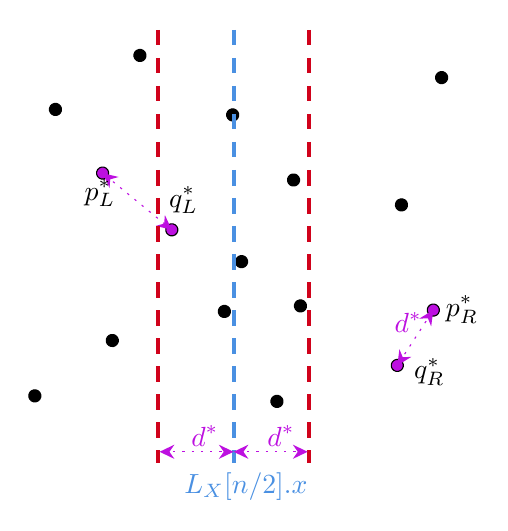
\begin{tikzpicture}[x=0.5pt,y=0.5pt,yscale=-1,xscale=1]
%uncomment if require: \path (0,347); %set diagram left start at 0, and has height of 347

%Flowchart: Connector [id:dp3585002987789013] 
\draw  [fill={rgb, 255:red, 0; green, 0; blue, 0 }  ,fill opacity=1 ] (229.06,171.88) .. controls (226.68,172.34) and (224.39,170.78) .. (223.94,168.41) .. controls (223.49,166.03) and (225.04,163.74) .. (227.42,163.29) .. controls (229.79,162.83) and (232.08,164.39) .. (232.54,166.77) .. controls (232.99,169.14) and (231.43,171.43) .. (229.06,171.88) -- cycle ;
%Flowchart: Connector [id:dp7980412079509043] 
\draw  [fill={rgb, 255:red, 0; green, 0; blue, 0 }  ,fill opacity=1 ] (94.58,61.88) .. controls (92.2,62.34) and (89.91,60.78) .. (89.46,58.41) .. controls (89,56.03) and (90.56,53.74) .. (92.94,53.29) .. controls (95.31,52.83) and (97.6,54.39) .. (98.05,56.77) .. controls (98.51,59.14) and (96.95,61.43) .. (94.58,61.88) -- cycle ;
%Flowchart: Connector [id:dp9736868983859984] 
\draw  [fill={rgb, 255:red, 0; green, 0; blue, 0 }  ,fill opacity=1 ] (155.62,22.88) .. controls (153.25,23.34) and (150.95,21.78) .. (150.5,19.41) .. controls (150.05,17.03) and (151.6,14.74) .. (153.98,14.29) .. controls (156.35,13.83) and (158.64,15.39) .. (159.1,17.77) .. controls (159.55,20.14) and (157.99,22.43) .. (155.62,22.88) -- cycle ;
%Flowchart: Connector [id:dp957649299032159] 
\draw  [fill={rgb, 255:red, 0; green, 0; blue, 0 }  ,fill opacity=1 ] (266.64,112.88) .. controls (264.27,113.34) and (261.98,111.78) .. (261.52,109.41) .. controls (261.07,107.03) and (262.63,104.74) .. (265,104.29) .. controls (267.37,103.83) and (269.67,105.39) .. (270.12,107.77) .. controls (270.57,110.14) and (269.02,112.43) .. (266.64,112.88) -- cycle ;
%Flowchart: Connector [id:dp9650319562783608] 
\draw  [fill={rgb, 255:red, 0; green, 0; blue, 0 }  ,fill opacity=1 ] (373.64,38.88) .. controls (371.27,39.34) and (368.98,37.78) .. (368.52,35.41) .. controls (368.07,33.03) and (369.63,30.74) .. (372,30.29) .. controls (374.37,29.83) and (376.67,31.39) .. (377.12,33.77) .. controls (377.57,36.14) and (376.02,38.43) .. (373.64,38.88) -- cycle ;
%Flowchart: Connector [id:dp1191629503329028] 
\draw  [color={rgb, 255:red, 0; green, 0; blue, 0 }  ,draw opacity=1 ][fill={rgb, 255:red, 189; green, 16; blue, 224 }  ,fill opacity=1 ] (178.64,148.88) .. controls (176.27,149.34) and (173.98,147.78) .. (173.52,145.41) .. controls (173.07,143.03) and (174.63,140.74) .. (177,140.29) .. controls (179.37,139.83) and (181.67,141.39) .. (182.12,143.77) .. controls (182.57,146.14) and (181.02,148.43) .. (178.64,148.88) -- cycle ;
%Flowchart: Connector [id:dp46368149090735455] 
\draw  [fill={rgb, 255:red, 189; green, 16; blue, 224 }  ,fill opacity=1 ] (341.62,246.88) .. controls (339.25,247.34) and (336.95,245.78) .. (336.5,243.41) .. controls (336.05,241.03) and (337.6,238.74) .. (339.98,238.29) .. controls (342.35,237.83) and (344.64,239.39) .. (345.1,241.77) .. controls (345.55,244.14) and (343.99,246.43) .. (341.62,246.88) -- cycle ;
%Flowchart: Connector [id:dp6008165035231083] 
\draw  [fill={rgb, 255:red, 0; green, 0; blue, 0 }  ,fill opacity=1 ] (216.64,207.88) .. controls (214.27,208.34) and (211.98,206.78) .. (211.52,204.41) .. controls (211.07,202.03) and (212.63,199.74) .. (215,199.29) .. controls (217.37,198.83) and (219.67,200.39) .. (220.12,202.77) .. controls (220.57,205.14) and (219.02,207.43) .. (216.64,207.88) -- cycle ;
%Flowchart: Connector [id:dp7362164431483738] 
\draw  [fill={rgb, 255:red, 0; green, 0; blue, 0 }  ,fill opacity=1 ] (222.64,65.84) .. controls (220.27,66.29) and (217.98,64.73) .. (217.52,62.36) .. controls (217.07,59.99) and (218.63,57.69) .. (221,57.24) .. controls (223.37,56.79) and (225.67,58.34) .. (226.12,60.72) .. controls (226.57,63.09) and (225.02,65.38) .. (222.64,65.84) -- cycle ;
%Straight Lines [id:da6529740224708328] 
\draw [color={rgb, 255:red, 74; green, 144; blue, 226 }  ,draw opacity=1 ][line width=1.5]  [dash pattern={on 5.63pt off 4.5pt}]  (222.5,0) -- (222.5,313) ;
%Flowchart: Connector [id:dp2239447293014194] 
\draw  [fill={rgb, 255:red, 0; green, 0; blue, 0 }  ,fill opacity=1 ] (135.64,228.88) .. controls (133.27,229.34) and (130.98,227.78) .. (130.52,225.41) .. controls (130.07,223.03) and (131.63,220.74) .. (134,220.29) .. controls (136.37,219.83) and (138.67,221.39) .. (139.12,223.77) .. controls (139.57,226.14) and (138.02,228.43) .. (135.64,228.88) -- cycle ;
%Flowchart: Connector [id:dp4443697198815304] 
\draw  [fill={rgb, 255:red, 0; green, 0; blue, 0 }  ,fill opacity=1 ] (254.64,272.88) .. controls (252.27,273.34) and (249.98,271.78) .. (249.52,269.41) .. controls (249.07,267.03) and (250.63,264.74) .. (253,264.29) .. controls (255.37,263.83) and (257.67,265.39) .. (258.12,267.77) .. controls (258.57,270.14) and (257.02,272.43) .. (254.64,272.88) -- cycle ;
%Flowchart: Connector [id:dp25292770923986996] 
\draw  [fill={rgb, 255:red, 189; green, 16; blue, 224 }  ,fill opacity=1 ] (128.64,107.88) .. controls (126.27,108.34) and (123.98,106.78) .. (123.52,104.41) .. controls (123.07,102.03) and (124.63,99.74) .. (127,99.29) .. controls (129.37,98.83) and (131.67,100.39) .. (132.12,102.77) .. controls (132.57,105.14) and (131.02,107.43) .. (128.64,107.88) -- cycle ;
%Flowchart: Connector [id:dp32241515903160844] 
\draw  [fill={rgb, 255:red, 0; green, 0; blue, 0 }  ,fill opacity=1 ] (79.64,268.88) .. controls (77.27,269.34) and (74.98,267.78) .. (74.52,265.41) .. controls (74.07,263.03) and (75.63,260.74) .. (78,260.29) .. controls (80.37,259.83) and (82.67,261.39) .. (83.12,263.77) .. controls (83.57,266.14) and (82.02,268.43) .. (79.64,268.88) -- cycle ;
%Flowchart: Connector [id:dp5412978107709706] 
\draw  [fill={rgb, 255:red, 0; green, 0; blue, 0 }  ,fill opacity=1 ] (344.64,130.88) .. controls (342.27,131.34) and (339.98,129.78) .. (339.52,127.41) .. controls (339.07,125.03) and (340.63,122.74) .. (343,122.29) .. controls (345.37,121.83) and (347.67,123.39) .. (348.12,125.77) .. controls (348.57,128.14) and (347.02,130.43) .. (344.64,130.88) -- cycle ;
%Flowchart: Connector [id:dp8188453538986455] 
\draw  [fill={rgb, 255:red, 189; green, 16; blue, 224 }  ,fill opacity=1 ] (367.64,206.88) .. controls (365.27,207.34) and (362.98,205.78) .. (362.52,203.41) .. controls (362.07,201.03) and (363.63,198.74) .. (366,198.29) .. controls (368.37,197.83) and (370.67,199.39) .. (371.12,201.77) .. controls (371.57,204.14) and (370.02,206.43) .. (367.64,206.88) -- cycle ;
%Straight Lines [id:da7981748798144619] 
\draw [color={rgb, 255:red, 189; green, 16; blue, 224 }  ,draw opacity=1 ] [dash pattern={on 0.84pt off 2.51pt}]  (130.14,105.49) -- (175.5,142.68) ;
\draw [shift={(177.82,144.59)}, rotate = 219.35] [fill={rgb, 255:red, 189; green, 16; blue, 224 }  ,fill opacity=1 ][line width=0.08]  [draw opacity=0] (10.72,-5.15) -- (0,0) -- (10.72,5.15) -- (7.12,0) -- cycle    ;
\draw [shift={(127.82,103.59)}, rotate = 39.35] [fill={rgb, 255:red, 189; green, 16; blue, 224 }  ,fill opacity=1 ][line width=0.08]  [draw opacity=0] (10.72,-5.15) -- (0,0) -- (10.72,5.15) -- (7.12,0) -- cycle    ;
%Straight Lines [id:da4570690123839587] 
\draw [color={rgb, 255:red, 189; green, 16; blue, 224 }  ,draw opacity=1 ] [dash pattern={on 0.84pt off 2.51pt}]  (342.44,240.07) -- (365.18,205.1) ;
\draw [shift={(366.82,202.59)}, rotate = 123.05] [fill={rgb, 255:red, 189; green, 16; blue, 224 }  ,fill opacity=1 ][line width=0.08]  [draw opacity=0] (10.72,-5.15) -- (0,0) -- (10.72,5.15) -- (7.12,0) -- cycle    ;
\draw [shift={(340.8,242.59)}, rotate = 303.05] [fill={rgb, 255:red, 189; green, 16; blue, 224 }  ,fill opacity=1 ][line width=0.08]  [draw opacity=0] (10.72,-5.15) -- (0,0) -- (10.72,5.15) -- (7.12,0) -- cycle    ;
%Straight Lines [id:da3441187372234148] 
\draw [color={rgb, 255:red, 208; green, 2; blue, 27 }  ,draw opacity=1 ][line width=1.5]  [dash pattern={on 5.63pt off 4.5pt}]  (168,0) -- (168,313) ;
%Straight Lines [id:da06503609524950982] 
\draw [color={rgb, 255:red, 208; green, 2; blue, 27 }  ,draw opacity=1 ][line width=1.5]  [dash pattern={on 5.63pt off 4.5pt}]  (277,0) -- (277,313) ;
%Straight Lines [id:da01899195473791948] 
\draw [color={rgb, 255:red, 189; green, 16; blue, 224 }  ,draw opacity=1 ] [dash pattern={on 0.84pt off 2.51pt}]  (172,305) -- (219.5,305) ;
\draw [shift={(222.5,305)}, rotate = 180] [fill={rgb, 255:red, 189; green, 16; blue, 224 }  ,fill opacity=1 ][line width=0.08]  [draw opacity=0] (10.72,-5.15) -- (0,0) -- (10.72,5.15) -- (7.12,0) -- cycle    ;
\draw [shift={(169,305)}, rotate = 0] [fill={rgb, 255:red, 189; green, 16; blue, 224 }  ,fill opacity=1 ][line width=0.08]  [draw opacity=0] (10.72,-5.15) -- (0,0) -- (10.72,5.15) -- (7.12,0) -- cycle    ;
%Straight Lines [id:da5930514326113744] 
\draw [color={rgb, 255:red, 189; green, 16; blue, 224 }  ,draw opacity=1 ] [dash pattern={on 0.84pt off 2.51pt}]  (225.5,305) -- (273,305) ;
\draw [shift={(276,305)}, rotate = 180] [fill={rgb, 255:red, 189; green, 16; blue, 224 }  ,fill opacity=1 ][line width=0.08]  [draw opacity=0] (10.72,-5.15) -- (0,0) -- (10.72,5.15) -- (7.12,0) -- cycle    ;
\draw [shift={(222.5,305)}, rotate = 0] [fill={rgb, 255:red, 189; green, 16; blue, 224 }  ,fill opacity=1 ][line width=0.08]  [draw opacity=0] (10.72,-5.15) -- (0,0) -- (10.72,5.15) -- (7.12,0) -- cycle    ;
%Flowchart: Connector [id:dp173337509020409] 
\draw  [fill={rgb, 255:red, 0; green, 0; blue, 0 }  ,fill opacity=1 ] (271.64,203.88) .. controls (269.27,204.34) and (266.98,202.78) .. (266.52,200.41) .. controls (266.07,198.03) and (267.63,195.74) .. (270,195.29) .. controls (272.37,194.83) and (274.67,196.39) .. (275.12,198.77) .. controls (275.57,201.14) and (274.02,203.43) .. (271.64,203.88) -- cycle ;

% Text Node
\draw (185,318.45) node [anchor=north west][inner sep=0.75pt]  [color={rgb, 255:red, 74; green, 144; blue, 226 }  ,opacity=1 ] [align=left] {$\displaystyle L_{X}[ n/2] .x$};
% Text Node
\draw (113,106.45) node [anchor=north west][inner sep=0.75pt]   [align=left] {$\displaystyle p_{L}^{*}$};
% Text Node
\draw (174,111.45) node [anchor=north west][inner sep=0.75pt]   [align=left] {$\displaystyle q_{L}^{*}$};
% Text Node
\draw (374,190.45) node [anchor=north west][inner sep=0.75pt]   [align=left] {$\displaystyle p_{R}^{*}$};
% Text Node
\draw (351,235.45) node [anchor=north west][inner sep=0.75pt]   [align=left] {$\displaystyle q_{R}^{*}$};
% Text Node
\draw (337,202.41) node [anchor=north west][inner sep=0.75pt]  [color={rgb, 255:red, 189; green, 16; blue, 224 }  ,opacity=1 ] [align=left] {$\displaystyle d^{*}$};
% Text Node
\draw (190,284.41) node [anchor=north west][inner sep=0.75pt]  [color={rgb, 255:red, 189; green, 16; blue, 224 }  ,opacity=1 ] [align=left] {$\displaystyle d^{*}$};
% Text Node
\draw (245,284.41) node [anchor=north west][inner sep=0.75pt]  [color={rgb, 255:red, 189; green, 16; blue, 224 }  ,opacity=1 ] [align=left] {$\displaystyle d^{*}$};


\end{tikzpicture}

}
\caption{Illustration of the band centered at line $x = L_X[n/2].x$ with width $2\cdot d^*$.}
\label{fig:band}
\end{figure}

Following above argument, we only need to consider points within a band
centered at the partition line, i.e., $x = L_X[2/n].x$.  See
Figure~\ref{fig:band}.  The width of this band is $2\cdot d^*$.
Any point outside this band must have a distance larger
than $d^*$ with any point on the other side.
Hence, if a pair spanning $L$ and $R$ have a distance smaller than $d^*$,
then both points must be in the band.

So we narrowed down the points to those in the band.
But we still cannot afford comparing all pairs in it.
Fortunately, we do not have to. In fact, for each point in the band,
we only \emph{need} to compare it to a \emph{constant} number of points.
This boils down the total number of comparisons to $\Theta(n)$.
Let's establish this key result. First, we need to create a sorted list
for points in the band, in ascending order of $y$-coordinates.
We denote this sorted list as $B_Y$.
The construction of $B_Y$, again, can be done by using the given sorted
list $P_Y$.  Specifically, we tranverse $P_Y$, and for each point $p$ in it,
determine if it is in the band, by testing if $|p.x - L_X[n/2].x| \le d^*$,
and if it is so, we put $p$ to the end of $B_Y$. The lemma given below states
the key conclusion: if two points are 12 positions or more apart in the
sorted list $B_Y$, then their distance is guaranteed to be larger than $d^*$.
With this lemma, in order to determine possible pair with distance smaller than $d^*$ in the band,
we just need to examine pairs $(B_Y[i], B_Y[j])$, where $j \le i + 12$.
The number of such pairs is certainly at most $12\cdot |B_Y|$, which is $\Theta(n)$.

\emph{Lemma.} If $j \ge i + 12$, then $dist(B_Y[i], B_Y[j]) \ge d^*$.

\begin{figure}[b!]
\centering{

\tikzset{every picture/.style={line width=0.75pt}} %set default line width to 0.75pt        

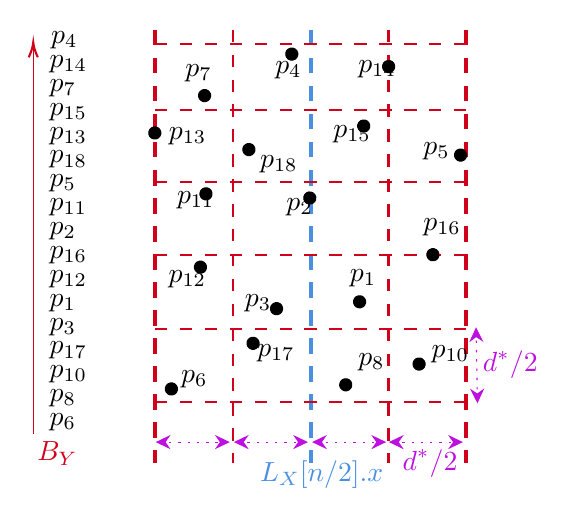
\begin{tikzpicture}[x=0.5pt,y=0.5pt,yscale=-1,xscale=1]
%uncomment if require: \path (0,377); %set diagram left start at 0, and has height of 377

%Straight Lines [id:da6529740224708328] 
\draw [color={rgb, 255:red, 74; green, 144; blue, 226 }  ,draw opacity=1 ][line width=1.5]  [dash pattern={on 5.63pt off 4.5pt}]  (222.5,7) -- (222.5,320) ;
%Straight Lines [id:da3441187372234148] 
\draw [color={rgb, 255:red, 208; green, 2; blue, 27 }  ,draw opacity=1 ][line width=0.75]  [dash pattern={on 4.5pt off 4.5pt}]  (166.25,7) -- (166.25,320) ;
%Straight Lines [id:da06503609524950982] 
\draw [color={rgb, 255:red, 208; green, 2; blue, 27 }  ,draw opacity=1 ][line width=0.75]  [dash pattern={on 4.5pt off 4.5pt}]  (278.75,7) -- (278.75,320) ;
%Straight Lines [id:da01899195473791948] 
\draw [color={rgb, 255:red, 189; green, 16; blue, 224 }  ,draw opacity=1 ] [dash pattern={on 0.84pt off 2.51pt}]  (170,305) -- (217.5,305) ;
\draw [shift={(220.5,305)}, rotate = 180] [fill={rgb, 255:red, 189; green, 16; blue, 224 }  ,fill opacity=1 ][line width=0.08]  [draw opacity=0] (10.72,-5.15) -- (0,0) -- (10.72,5.15) -- (7.12,0) -- cycle    ;
\draw [shift={(167,305)}, rotate = 0] [fill={rgb, 255:red, 189; green, 16; blue, 224 }  ,fill opacity=1 ][line width=0.08]  [draw opacity=0] (10.72,-5.15) -- (0,0) -- (10.72,5.15) -- (7.12,0) -- cycle    ;
%Straight Lines [id:da5930514326113744] 
\draw [color={rgb, 255:red, 189; green, 16; blue, 224 }  ,draw opacity=1 ] [dash pattern={on 0.84pt off 2.51pt}]  (226.5,305) -- (274,305) ;
\draw [shift={(277,305)}, rotate = 180] [fill={rgb, 255:red, 189; green, 16; blue, 224 }  ,fill opacity=1 ][line width=0.08]  [draw opacity=0] (10.72,-5.15) -- (0,0) -- (10.72,5.15) -- (7.12,0) -- cycle    ;
\draw [shift={(223.5,305)}, rotate = 0] [fill={rgb, 255:red, 189; green, 16; blue, 224 }  ,fill opacity=1 ][line width=0.08]  [draw opacity=0] (10.72,-5.15) -- (0,0) -- (10.72,5.15) -- (7.12,0) -- cycle    ;
%Straight Lines [id:da9199871224664768] 
\draw [color={rgb, 255:red, 208; green, 2; blue, 27 }  ,draw opacity=1 ][line width=1.5]  [dash pattern={on 5.63pt off 4.5pt}]  (110,7) -- (110,320) ;
%Straight Lines [id:da313545184348601] 
\draw [color={rgb, 255:red, 208; green, 2; blue, 27 }  ,draw opacity=1 ][line width=1.5]  [dash pattern={on 5.63pt off 4.5pt}]  (335,7) -- (335,320) ;
%Straight Lines [id:da008171567906934074] 
\draw [color={rgb, 255:red, 189; green, 16; blue, 224 }  ,draw opacity=1 ] [dash pattern={on 0.84pt off 2.51pt}]  (113.5,305) -- (161,305) ;
\draw [shift={(164,305)}, rotate = 180] [fill={rgb, 255:red, 189; green, 16; blue, 224 }  ,fill opacity=1 ][line width=0.08]  [draw opacity=0] (10.72,-5.15) -- (0,0) -- (10.72,5.15) -- (7.12,0) -- cycle    ;
\draw [shift={(110.5,305)}, rotate = 0] [fill={rgb, 255:red, 189; green, 16; blue, 224 }  ,fill opacity=1 ][line width=0.08]  [draw opacity=0] (10.72,-5.15) -- (0,0) -- (10.72,5.15) -- (7.12,0) -- cycle    ;
%Straight Lines [id:da5296316037034452] 
\draw [color={rgb, 255:red, 189; green, 16; blue, 224 }  ,draw opacity=1 ] [dash pattern={on 0.84pt off 2.51pt}]  (282,305) -- (329.5,305) ;
\draw [shift={(332.5,305)}, rotate = 180] [fill={rgb, 255:red, 189; green, 16; blue, 224 }  ,fill opacity=1 ][line width=0.08]  [draw opacity=0] (10.72,-5.15) -- (0,0) -- (10.72,5.15) -- (7.12,0) -- cycle    ;
\draw [shift={(279,305)}, rotate = 0] [fill={rgb, 255:red, 189; green, 16; blue, 224 }  ,fill opacity=1 ][line width=0.08]  [draw opacity=0] (10.72,-5.15) -- (0,0) -- (10.72,5.15) -- (7.12,0) -- cycle    ;
%Straight Lines [id:da4429916887913099] 
\draw [color={rgb, 255:red, 208; green, 2; blue, 27 }  ,draw opacity=1 ][line width=0.75]  [dash pattern={on 4.5pt off 4.5pt}]  (110,276) -- (335,276) ;
%Straight Lines [id:da6783093940157634] 
\draw [color={rgb, 255:red, 208; green, 2; blue, 27 }  ,draw opacity=1 ][line width=0.75]  [dash pattern={on 4.5pt off 4.5pt}]  (110,223) -- (335,223) ;
%Straight Lines [id:da3395926668100431] 
\draw [color={rgb, 255:red, 208; green, 2; blue, 27 }  ,draw opacity=1 ][line width=0.75]  [dash pattern={on 4.5pt off 4.5pt}]  (110,170) -- (335,170) ;
%Straight Lines [id:da11772188438625031] 
\draw [color={rgb, 255:red, 208; green, 2; blue, 27 }  ,draw opacity=1 ][line width=0.75]  [dash pattern={on 4.5pt off 4.5pt}]  (110,117) -- (335,117) ;
%Straight Lines [id:da5874985603564619] 
\draw [color={rgb, 255:red, 208; green, 2; blue, 27 }  ,draw opacity=1 ][line width=0.75]  [dash pattern={on 4.5pt off 4.5pt}]  (110,65) -- (335,65) ;
%Straight Lines [id:da706623823441126] 
\draw [color={rgb, 255:red, 208; green, 2; blue, 27 }  ,draw opacity=1 ][line width=0.75]  [dash pattern={on 4.5pt off 4.5pt}]  (110,17) -- (335,17) ;
%Straight Lines [id:da8387514930702964] 
\draw [color={rgb, 255:red, 189; green, 16; blue, 224 }  ,draw opacity=1 ] [dash pattern={on 0.84pt off 2.51pt}]  (342.05,225) -- (342.95,274) ;
\draw [shift={(343,277)}, rotate = 268.96] [fill={rgb, 255:red, 189; green, 16; blue, 224 }  ,fill opacity=1 ][line width=0.08]  [draw opacity=0] (10.72,-5.15) -- (0,0) -- (10.72,5.15) -- (7.12,0) -- cycle    ;
\draw [shift={(342,222)}, rotate = 88.96] [fill={rgb, 255:red, 189; green, 16; blue, 224 }  ,fill opacity=1 ][line width=0.08]  [draw opacity=0] (10.72,-5.15) -- (0,0) -- (10.72,5.15) -- (7.12,0) -- cycle    ;
%Flowchart: Connector [id:dp8923414673582244] 
\draw  [fill={rgb, 255:red, 0; green, 0; blue, 0 }  ,fill opacity=1 ] (248.64,267.88) .. controls (246.27,268.34) and (243.98,266.78) .. (243.52,264.41) .. controls (243.07,262.03) and (244.63,259.74) .. (247,259.29) .. controls (249.37,258.83) and (251.67,260.39) .. (252.12,262.77) .. controls (252.57,265.14) and (251.02,267.43) .. (248.64,267.88) -- cycle ;
%Flowchart: Connector [id:dp6825138981911604] 
\draw  [fill={rgb, 255:red, 0; green, 0; blue, 0 }  ,fill opacity=1 ] (181.64,237.88) .. controls (179.27,238.34) and (176.98,236.78) .. (176.52,234.41) .. controls (176.07,232.03) and (177.63,229.74) .. (180,229.29) .. controls (182.37,228.83) and (184.67,230.39) .. (185.12,232.77) .. controls (185.57,235.14) and (184.02,237.43) .. (181.64,237.88) -- cycle ;
%Flowchart: Connector [id:dp4157984407010722] 
\draw  [fill={rgb, 255:red, 0; green, 0; blue, 0 }  ,fill opacity=1 ] (122.64,270.88) .. controls (120.27,271.34) and (117.98,269.78) .. (117.52,267.41) .. controls (117.07,265.03) and (118.63,262.74) .. (121,262.29) .. controls (123.37,261.83) and (125.67,263.39) .. (126.12,265.77) .. controls (126.57,268.14) and (125.02,270.43) .. (122.64,270.88) -- cycle ;
%Flowchart: Connector [id:dp8333199543319949] 
\draw  [fill={rgb, 255:red, 0; green, 0; blue, 0 }  ,fill opacity=1 ] (301.64,252.88) .. controls (299.27,253.34) and (296.98,251.78) .. (296.52,249.41) .. controls (296.07,247.03) and (297.63,244.74) .. (300,244.29) .. controls (302.37,243.83) and (304.67,245.39) .. (305.12,247.77) .. controls (305.57,250.14) and (304.02,252.43) .. (301.64,252.88) -- cycle ;
%Flowchart: Connector [id:dp36334472410839813] 
\draw  [fill={rgb, 255:red, 0; green, 0; blue, 0 }  ,fill opacity=1 ] (258.64,207.88) .. controls (256.27,208.34) and (253.98,206.78) .. (253.52,204.41) .. controls (253.07,202.03) and (254.63,199.74) .. (257,199.29) .. controls (259.37,198.83) and (261.67,200.39) .. (262.12,202.77) .. controls (262.57,205.14) and (261.02,207.43) .. (258.64,207.88) -- cycle ;
%Flowchart: Connector [id:dp09374517288306172] 
\draw  [fill={rgb, 255:red, 0; green, 0; blue, 0 }  ,fill opacity=1 ] (198.64,212.88) .. controls (196.27,213.34) and (193.98,211.78) .. (193.52,209.41) .. controls (193.07,207.03) and (194.63,204.74) .. (197,204.29) .. controls (199.37,203.83) and (201.67,205.39) .. (202.12,207.77) .. controls (202.57,210.14) and (201.02,212.43) .. (198.64,212.88) -- cycle ;
%Flowchart: Connector [id:dp2674555355524125] 
\draw  [fill={rgb, 255:red, 0; green, 0; blue, 0 }  ,fill opacity=1 ] (143.64,182.88) .. controls (141.27,183.34) and (138.98,181.78) .. (138.52,179.41) .. controls (138.07,177.03) and (139.63,174.74) .. (142,174.29) .. controls (144.37,173.83) and (146.67,175.39) .. (147.12,177.77) .. controls (147.57,180.14) and (146.02,182.43) .. (143.64,182.88) -- cycle ;
%Flowchart: Connector [id:dp4988189914468546] 
\draw  [fill={rgb, 255:red, 0; green, 0; blue, 0 }  ,fill opacity=1 ] (311.64,173.88) .. controls (309.27,174.34) and (306.98,172.78) .. (306.52,170.41) .. controls (306.07,168.03) and (307.63,165.74) .. (310,165.29) .. controls (312.37,164.83) and (314.67,166.39) .. (315.12,168.77) .. controls (315.57,171.14) and (314.02,173.43) .. (311.64,173.88) -- cycle ;
%Flowchart: Connector [id:dp6877256898622583] 
\draw  [fill={rgb, 255:red, 0; green, 0; blue, 0 }  ,fill opacity=1 ] (222.64,132.88) .. controls (220.27,133.34) and (217.98,131.78) .. (217.52,129.41) .. controls (217.07,127.03) and (218.63,124.74) .. (221,124.29) .. controls (223.37,123.83) and (225.67,125.39) .. (226.12,127.77) .. controls (226.57,130.14) and (225.02,132.43) .. (222.64,132.88) -- cycle ;
%Flowchart: Connector [id:dp7258428027313548] 
\draw  [fill={rgb, 255:red, 0; green, 0; blue, 0 }  ,fill opacity=1 ] (147.64,129.88) .. controls (145.27,130.34) and (142.98,128.78) .. (142.52,126.41) .. controls (142.07,124.03) and (143.63,121.74) .. (146,121.29) .. controls (148.37,120.83) and (150.67,122.39) .. (151.12,124.77) .. controls (151.57,127.14) and (150.02,129.43) .. (147.64,129.88) -- cycle ;
%Flowchart: Connector [id:dp4759673781795757] 
\draw  [fill={rgb, 255:red, 0; green, 0; blue, 0 }  ,fill opacity=1 ] (331.64,101.88) .. controls (329.27,102.34) and (326.98,100.78) .. (326.52,98.41) .. controls (326.07,96.03) and (327.63,93.74) .. (330,93.29) .. controls (332.37,92.83) and (334.67,94.39) .. (335.12,96.77) .. controls (335.57,99.14) and (334.02,101.43) .. (331.64,101.88) -- cycle ;
%Flowchart: Connector [id:dp8213326726444833] 
\draw  [fill={rgb, 255:red, 0; green, 0; blue, 0 }  ,fill opacity=1 ] (261.64,80.88) .. controls (259.27,81.34) and (256.98,79.78) .. (256.52,77.41) .. controls (256.07,75.03) and (257.63,72.74) .. (260,72.29) .. controls (262.37,71.83) and (264.67,73.39) .. (265.12,75.77) .. controls (265.57,78.14) and (264.02,80.43) .. (261.64,80.88) -- cycle ;
%Flowchart: Connector [id:dp19921591820820672] 
\draw  [fill={rgb, 255:red, 0; green, 0; blue, 0 }  ,fill opacity=1 ] (178.64,97.88) .. controls (176.27,98.34) and (173.98,96.78) .. (173.52,94.41) .. controls (173.07,92.03) and (174.63,89.74) .. (177,89.29) .. controls (179.37,88.83) and (181.67,90.39) .. (182.12,92.77) .. controls (182.57,95.14) and (181.02,97.43) .. (178.64,97.88) -- cycle ;
%Flowchart: Connector [id:dp45521771767073826] 
\draw  [fill={rgb, 255:red, 0; green, 0; blue, 0 }  ,fill opacity=1 ] (110.64,85.88) .. controls (108.27,86.34) and (105.98,84.78) .. (105.52,82.41) .. controls (105.07,80.03) and (106.63,77.74) .. (109,77.29) .. controls (111.37,76.83) and (113.67,78.39) .. (114.12,80.77) .. controls (114.57,83.14) and (113.02,85.43) .. (110.64,85.88) -- cycle ;
%Flowchart: Connector [id:dp6969160770264389] 
\draw  [fill={rgb, 255:red, 0; green, 0; blue, 0 }  ,fill opacity=1 ] (279.64,37.88) .. controls (277.27,38.34) and (274.98,36.78) .. (274.52,34.41) .. controls (274.07,32.03) and (275.63,29.74) .. (278,29.29) .. controls (280.37,28.83) and (282.67,30.39) .. (283.12,32.77) .. controls (283.57,35.14) and (282.02,37.43) .. (279.64,37.88) -- cycle ;
%Flowchart: Connector [id:dp17503792181776967] 
\draw  [fill={rgb, 255:red, 0; green, 0; blue, 0 }  ,fill opacity=1 ] (209.64,28.88) .. controls (207.27,29.34) and (204.98,27.78) .. (204.52,25.41) .. controls (204.07,23.03) and (205.63,20.74) .. (208,20.29) .. controls (210.37,19.83) and (212.67,21.39) .. (213.12,23.77) .. controls (213.57,26.14) and (212.02,28.43) .. (209.64,28.88) -- cycle ;
%Flowchart: Connector [id:dp7711561658315957] 
\draw  [fill={rgb, 255:red, 0; green, 0; blue, 0 }  ,fill opacity=1 ] (146.64,58.88) .. controls (144.27,59.34) and (141.98,57.78) .. (141.52,55.41) .. controls (141.07,53.03) and (142.63,50.74) .. (145,50.29) .. controls (147.37,49.83) and (149.67,51.39) .. (150.12,53.77) .. controls (150.57,56.14) and (149.02,58.43) .. (146.64,58.88) -- cycle ;
%Straight Lines [id:da023124782613843764] 
\draw [color={rgb, 255:red, 208; green, 2; blue, 27 }  ,draw opacity=1 ]   (22,299) -- (22,18) ;
\draw [shift={(22,16)}, rotate = 90] [color={rgb, 255:red, 208; green, 2; blue, 27 }  ,draw opacity=1 ][line width=0.75]    (10.93,-3.29) .. controls (6.95,-1.4) and (3.31,-0.3) .. (0,0) .. controls (3.31,0.3) and (6.95,1.4) .. (10.93,3.29)   ;

% Text Node
\draw (184,316.45) node [anchor=north west][inner sep=0.75pt]  [color={rgb, 255:red, 74; green, 144; blue, 226 }  ,opacity=1 ] [align=left] {$\displaystyle L_{X}[ n/2] .x$};
% Text Node
\draw (287,308.41) node [anchor=north west][inner sep=0.75pt]  [color={rgb, 255:red, 189; green, 16; blue, 224 }  ,opacity=1 ] [align=left] {$\displaystyle d^{*} /2$};
% Text Node
\draw (345,237.41) node [anchor=north west][inner sep=0.75pt]  [color={rgb, 255:red, 189; green, 16; blue, 224 }  ,opacity=1 ] [align=left] {$\displaystyle d^{*} /2$};
% Text Node
\draw (127,251.45) node [anchor=north west][inner sep=0.75pt]   [align=left] {$\displaystyle p_{6}$};
% Text Node
\draw (182,232.29) node [anchor=north west][inner sep=0.75pt]   [align=left] {$\displaystyle p_{17}$};
% Text Node
\draw (255,239.29) node [anchor=north west][inner sep=0.75pt]   [align=left] {$\displaystyle p_{8}$};
% Text Node
\draw (308,233.29) node [anchor=north west][inner sep=0.75pt]   [align=left] {$\displaystyle p_{10}$};
% Text Node
\draw (249,178.29) node [anchor=north west][inner sep=0.75pt]   [align=left] {$\displaystyle p_{1}$};
% Text Node
\draw (173,196.29) node [anchor=north west][inner sep=0.75pt]   [align=left] {$\displaystyle p_{3}$};
% Text Node
\draw (118,179.29) node [anchor=north west][inner sep=0.75pt]   [align=left] {$\displaystyle p_{12}$};
% Text Node
\draw (124,122.29) node [anchor=north west][inner sep=0.75pt]   [align=left] {$\displaystyle p_{11}$};
% Text Node
\draw (203,127.29) node [anchor=north west][inner sep=0.75pt]   [align=left] {$\displaystyle p_{2}$};
% Text Node
\draw (237,74.29) node [anchor=north west][inner sep=0.75pt]   [align=left] {$\displaystyle p_{15}$};
% Text Node
\draw (302,86.29) node [anchor=north west][inner sep=0.75pt]   [align=left] {$\displaystyle p_{5}$};
% Text Node
\draw (255,27.29) node [anchor=north west][inner sep=0.75pt]   [align=left] {$\displaystyle p_{14}$};
% Text Node
\draw (195,28.29) node [anchor=north west][inner sep=0.75pt]   [align=left] {$\displaystyle p_{4}$};
% Text Node
\draw (130,30.29) node [anchor=north west][inner sep=0.75pt]   [align=left] {$\displaystyle p_{7}$};
% Text Node
\draw (184.12,95.77) node [anchor=north west][inner sep=0.75pt]   [align=left] {$\displaystyle p_{18}$};
% Text Node
\draw (118.12,75.77) node [anchor=north west][inner sep=0.75pt]   [align=left] {$\displaystyle p_{13}$};
% Text Node
\draw (302,141.29) node [anchor=north west][inner sep=0.75pt]   [align=left] {$\displaystyle p_{16}$};
% Text Node
\draw (32,282.45) node [anchor=north west][inner sep=0.75pt]   [align=left] {$\displaystyle p_{6}$};
% Text Node
\draw (32,230.73) node [anchor=north west][inner sep=0.75pt]   [align=left] {$\displaystyle p_{17}$};
% Text Node
\draw (32,265.23) node [anchor=north west][inner sep=0.75pt]   [align=left] {$\displaystyle p_{8}$};
% Text Node
\draw (32,247.98) node [anchor=north west][inner sep=0.75pt]   [align=left] {$\displaystyle p_{10}$};
% Text Node
\draw (32,196.23) node [anchor=north west][inner sep=0.75pt]   [align=left] {$\displaystyle p_{1}$};
% Text Node
\draw (32,213.48) node [anchor=north west][inner sep=0.75pt]   [align=left] {$\displaystyle p_{3}$};
% Text Node
\draw (32,178.98) node [anchor=north west][inner sep=0.75pt]   [align=left] {$\displaystyle p_{12}$};
% Text Node
\draw (32,127.23) node [anchor=north west][inner sep=0.75pt]   [align=left] {$\displaystyle p_{11}$};
% Text Node
\draw (32,144.48) node [anchor=north west][inner sep=0.75pt]   [align=left] {$\displaystyle p_{2}$};
% Text Node
\draw (32,58.23) node [anchor=north west][inner sep=0.75pt]   [align=left] {$\displaystyle p_{15}$};
% Text Node
\draw (32,109.98) node [anchor=north west][inner sep=0.75pt]   [align=left] {$\displaystyle p_{5}$};
% Text Node
\draw (32,23.73) node [anchor=north west][inner sep=0.75pt]   [align=left] {$\displaystyle p_{14}$};
% Text Node
\draw (33,6.48) node [anchor=north west][inner sep=0.75pt]   [align=left] {$\displaystyle p_{4}$};
% Text Node
\draw (32,40.98) node [anchor=north west][inner sep=0.75pt]   [align=left] {$\displaystyle p_{7}$};
% Text Node
\draw (32,92.73) node [anchor=north west][inner sep=0.75pt]   [align=left] {$\displaystyle p_{18}$};
% Text Node
\draw (32,75.48) node [anchor=north west][inner sep=0.75pt]   [align=left] {$\displaystyle p_{13}$};
% Text Node
\draw (32,161.73) node [anchor=north west][inner sep=0.75pt]   [align=left] {$\displaystyle p_{16}$};
% Text Node
\draw (23,303) node [anchor=north west][inner sep=0.75pt]  [color={rgb, 255:red, 208; green, 2; blue, 27 }  ,opacity=1 ] [align=left] {$\displaystyle B_{Y}$};


\end{tikzpicture}

}
\caption{Illustration the proof of above lemma.}
\label{fig:boxes}
\end{figure}

We now prove above lemma. We partition the band into squares of size $d^*/2 \times d^*/2$.
See Figure~\ref{fig:boxes}. We first prove that, there is at most 1 point in each box~(including its boundary).
Suppose conversely that there are two points, $p$ and $q$, in a box.
Then the distance between them $dist(p,q) \le d^*/2\cdot \sqrt{2} < d^*$.
This is a contradiction, since each box is entirely inside either left side or the right side,
and we know that the closest pair not spanning two sides is $d^*$.
Next, if $j \ge i + 12$, then $B_Y[j]$ is at least three layers of boxes above $B_Y[i]$.
This is because, each layer contains 4 boxes, and therefore at most 4 points can be in them.
Hence if $B_Y[i]$ is in layer-$l$, then $B_Y[j]$ must be in layer-$(l + 3)$ or higher.
The height of each layer is $d^*/2$. The vertical distance between $B_Y[i]$ and $B_Y[j]$
is hence larger than $d^*$; therefore, their distance $dist(B_Y[i], B_Y[j]) > d^*$.

The complete algorithm is given below in pseudo-code.

\begin{minipage}{0.8\textwidth}
	\aaA {4}{Algorithm~\#2~($P[1\cdots n]$)}\xxx
	\aab {sort $P$ according to $x$-coordinates to obtain $P_X$;}\xxx
	\aab {sort $P$ according to $y$-coordinates to obtain $P_Y$;}\xxx
	\aab {return DC-closest-pair~($P_X$, $P_Y$);}\xxx
	\aaa {end algorithm;}\xxx
\end{minipage}

\begin{minipage}{0.8\textwidth}
	\aaA {24}{function DC-closest-pair~($P_X$, $P_Y$)}\xxx
	\aab {if $|P_X| \le 3$: enumerate all pairs to find the closest pair and return it;}\xxx
	\aab {$L_X = P_X[1\cdots n/2]$, $R_X = P_X[n/2 + 1\cdots n]$; }\xxx
	\aab {init $L_Y$ and $R_Y$ as empty lists; }\xxx
	\aab {let $x^* = L_X[n/2].x$; }\xxx
	\aaB {3}{for $i=1$ to $|P_Y|$}\xxx
	\aac {if $P_Y[i].x \le x^*$: add $P_Y[i]$ to the end of $L_Y$;}\xxx
	\aac {else: add $P_Y[i]$ to the end of $R_Y$;}\xxx
	\aab {end}\xxx
	\aab {$(p^*_L, q^*_L)$ = DC-closest-pair~($L_X, L_Y$);}\xxx
	\aab {$(p^*_R, q^*_R)$ = DC-closest-pair~($R_X, R_Y$);}\xxx
	\aab {$d^* = \min\{dist(p^*_L, q^*_L), dist(p^*_R, q^*_R)\}$;}\xxx
	\aab {$(p^*,q^*) = \arg\min\{dist(p^*_L, q^*_L), dist(p^*_R, q^*_R)\}$, to store the closest pair found from two halves;}\xxx
	\aab {init $B_Y$ as an empty list; }\xxx
	\aaB {2}{for $i=1$ to $|P_Y|$}\xxx
	\aac {if $|P_Y[i].x - x^*| \le d^*$: add $P_Y[i]$ to the end of $B_Y$;}\xxx
	\aab {end}\xxx
	\aaB {5}{for $i=1$ to $|B_Y|$}\xxx
	\aaC {3}{for $j=i + 1$ to $i + 12$}\xxx
	\aad {$d = dist(B_Y[i], B_Y[j])$;}\xxx
	\aad {if $d<d^*$: $d^* = d$, $p^* = B_X[i]$, $q^* = B_Y[j]$;}\xxx
	\aac {end}\xxx
	\aab {end}\xxx
	\aab {return $(p^*, q^*)$; }\xxx
	\aaa {end algorithm;}\xxx
\end{minipage}


Let's analyze the time complexity.
Let $T(n)$ be running time of DC-closest-pair~($P_X$, $P_Y$) when $|P_X| = |P_Y| = n$.
In DC-closest-pair function, the two recursive calls takes $2\cdot T(n/2)$ time;
the rest takes $\Theta(n)$ time.
Therefore, the recurrence is $T(n) = 2\cdot T(n/2) + \Theta(n)$ which gives $T(n) = \Theta(n\cdot \log n)$.
The entire algorithm~\#2 is therefore also takes $\Theta(n\cdot \log n)$ time since the two sorts takes
$\Theta(n\cdot \log n)$ as well.

